%%%%%%%%%%%%%%%%%%%%%%%%%%%%%%%%%%%%%%%%%%%%%%%%
% Compilation
%%%%%%%%%%%%%%%%%%%%%%%%%%%%%%%%%%%%%%%%%%%%%%%%

In this section we will show an outline of the Casanova compiler. In Fig. \ref{fig:compilation_process} we can see that compilation is a four step process.

In the first step we parse the program source code. The output is an AST which represents the program, with the rules and types as annotations.

The AST is fed to the type checker, which makes sure that the program does not contain incorrect operations. It makes sure that no duplication of \texttt{Rule T} values happens, which would cause inconsistencies when applying rules. The type checker also makes sure that behaviors are typed correctly, thereby ensuring that all behaviors are typed as \texttt{Safebehavior} and thus they do not cycle indefinitely without invoking \texttt{yield}.

The resulting AST is then processed by the F\# translator, which generates F\# code that defines the state and entity types and which implements the semantic function.

The F\# translator also performs some optimizations which we will discuss in the next paragraph.

Finally, the resulting F\# program is compiled by the standard F\# compiler thereby generating a library which can then be used as the game engine for an XNA (Windows PCs, Xbox 360 or Windows Phone 7) or MonoTouch (iPad, iPhone or Android) game.

\begin{figure}
\begin{center}
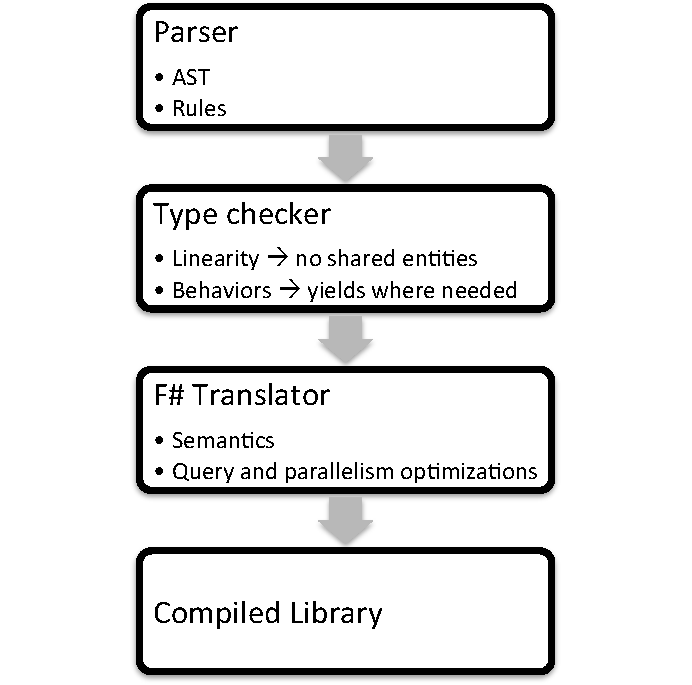
\includegraphics[scale=0.75]{compilation_process.pdf}
\end{center}
\caption{Compilation process}
\label{fig:compilation_process}
\end{figure}


\paragraph{Optimization}

Casanova performs three main optimizations.

The first optimization is a very simple one: memory recycling; even if simple, it can prove very effective in all those platforms (such as the Xbox 360) with a slow garbage collector. Memory recycling means that \texttt{Rule T} fields allocate a double buffer for storing both the $\mathtt{m}[r \rightarrow v]$ value and the $\mathtt{m}[r \Rightarrow v]$ value. Applying the $\oplus \mathtt{m}$ operator simply requires swapping the two buffers. The \texttt{Rule T} datatype is defined as:

\begin{lstlisting}
type Rule<'a> =
  {
    Values              : 'a[]
    FrameIndex          : int ref
  }
  member private this.ValueIndex
    with get() = this.FrameIndex.Value % this.NumValues
  member private this.ValueIndex' 
    with get() = (this.FrameIndex.Value + 1) % this.NumValues
  member this.Value
    with get() = this.Values.[this.ValueIndex]
    and set v' = this.Values.[this.ValueIndex] <- v'
  member this.Value'
    with get() = this.Values.[this.ValueIndex']
    and set v' = this.Values.[this.ValueIndex'] <- v'
\end{lstlisting}

all \texttt{Rule T}'s share the same reference to the current frame index. Whenever we wish to swap the references (that is when we apply the $\oplus$ function) then we just increment the \texttt{FrameIndex} without any need for traversing the entire state to manually set all \texttt{Rule T}'s.

This optimization can be extended to tables: at the beginning of each update, all values of type \texttt{Rule (Table T)} get their \texttt{Value'} cleared; clearing a table does not deallocate its elements: rather, it simply sets the counter of elements to zero, while keeping the previous memory allocated.

This strategy helps reducing the amount of garbage collection needed, sometimes giving large speedups as we can see in Section \ref{sec:benchmarks}.


The second optimization takes advantage of the static constraint that rules are linear: this means that no rules write the same memory location. We also know that rules may not freely write any references. These two facts guarantee thread safety, that is we may run or rules in parallel. Casanova dynamically allocates twice as many threads as the number of cores of the machine. Threads are only used to process lists of entities in the \texttt{GameState}, but no further multi-threading is performed: if an entity should contain many sub-entities those will all be processed sequentially in the same thread. This is needed to avoid creating too many threads; an excessive number of threads may even cause so much overhead that the benefits of parallelization are inferior to the losses in performance caused by the cost of threads.

The $i^{th}$ thread of $n$ will process the $i^{th}$ portion of each top-level table of the game state. This means that if the state is defined as:

\begin{lstlisting}
type GameState = 
  {
    Asteroids   : Table Asteroid
    Projectiles : Table Projectile
  }
\end{lstlisting}

then the $i^{th}$ thread will run the function:

\begin{lstlisting}
let thread state n i =
  for j = i * state.Asteroids.Count / n 
      to (i+1) * state.Asteroids.Count / n do
    update state.Asteroids.[j]
  for j = i * state.Projectiles.Count / n 
      to (i+1) * state.Projectiles.Count / n do
    update state.Projectiles.[j]
\end{lstlisting}

Unless the number of entities is very small or behaviors are very complex and computationally intensive, then the gains obtained by parallelization can be very high; the best results may even divide the duration of a tick by the number of threads, even if this is rarely the case.


The final optimization is query optimization. Nested list comprehensions (also known as ``joins'' in the field of databases) can have high computational costs; for example, the query:

\begin{lstlisting}
type Asteroid =
  {
    CollidingProjectiles 
      : Rule(Table(Foreign(Projectile)))
      :: \(state,self) -> [p | p <- state.Projectiles, collides(self,p)]     
  }
\end{lstlisting}

has a computational complexity of $O(n_p \times n_a) = O(n^2)$, where $n_p$ is the number of projectiles, $n_a$ is the number of asteroids and $n$ is the maximum between the two. Such a complexity is unacceptable when we start having a large number of asteroids and projectiles, because it may severely limit the maximum number of entities supported by the game.

We use the same physical optimization techniques used in modern databases: we build an index to speed up our collision detection. In particular, we observe that most asteroids and projectiles are so far away that testing them for collision does not make sense. We partition the space of the playing area into various blocks and we assign all our projectiles to the blocks they belong to; this operation costs $O(n_p)$ if blocks are a uniform grid and $O(n_p \log n_p)$ if blocks are of variable size and represented with a tree. For each asteroid, we find the blocks it belongs to ($O(n_a)$ or $O(n_a \log n_a)$) and then check for collisions only with the projectiles in those blocks. The final cost of the operation is $O(n)$ for hash maps and $O(n \log n)$ for trees.

An example hash map optimization could be the following. We add the following declaration to the game state:

\begin{lstlisting}
type GameState = 
  {
    ...
    Blocks   : Block[][]
  }
\end{lstlisting}

where a \texttt{Block} contains a list of projectiles.

In the update function we start by clearing the \texttt{Blocks} index and we fill it again with the updated projectiles:

\begin{lstlisting}
let update_state (state:GameState) (dt:float32) =
  for b in state.Blocks do
    b.Clear()
  
  for p in state.Projectiles do
    for b in p.Blocks do
      b.Add p
\end{lstlisting}

Benchmarks show that the costs of rebuilding the index are similar to modifying it, especially for trees. In this sense we confirm a similar result found in.

Collision detection will now become:

\begin{lstlisting}
let update_asteroid (state:GameState) 
                    (self:Asteroid) 
                    (dt:float32) =
  for b in self.Blocks do
    for p in b.Projectiles do
      if collides self p then
        self.CollidingProjectiles.Add p
\end{lstlisting}

A small bottleneck of this computation is the clearing phase, because it forces us to iterate all the blocks (which may be a large number for increased optimization) even if most of those are empty. For this reason, we further augment the state to track those blocks that contain projectiles (and thus which need clearing):

\begin{lstlisting}
type GameState = 
  {
    ...
    NonEmptyBlocks  : Table (BlockIndex)
  }
\end{lstlisting}

Now the update function becomes:

\begin{lstlisting}
let update_state (state:GameState) (dt:float32) =
  for bi in state.NonEmptyBlocks do
    state.Blocks.[bi].Clear()
  
  for p in state.Projectiles do
    for b in p.Blocks do
      b.Add p
      state.NonEmptyBlocks.Add b.Index
\end{lstlisting}

We must stress the importance of this last optimization. By having a function of quadratic complexity in the number of entities we are forcing our game to run with a maximum number of entities. Less entities often make for a less compelling game, because the world is less complex and the challenges are smaller. This class of optimizations allows the game performance to be less dependent on the number of entities. This means that we may design grander worlds with thousands of units and \textit{with no additional development complexity}.